
\section{Grayscale}

\begin{frame}
    \frametitle{Grayscale}

    \begin{itemize}
        \item Wandelt drei Farbwerte in einen Schwarz-Weis-Wert um \pause
        \item Zwei verschiedene Formeln \pause
        \item OpenCV\only<3->{\footnote{OpenCV wurde in der Implementierung verwendet}}: $ f(r, g, b) = 0.21r + 0.72g + 0.07b $  \pause
        \item Luminosity: $ f(r, g, b) =  0.299r + 0.587g + 0.114b $ \pause
    \end{itemize}
\end{frame}


\begin{frame}
    \frametitle{Grayscale - Ergebnisse 1}

    \begin{itemize}
        \item dice.png
        \item 800 x 600
        \item 295 KB
    \end{itemize}

    \hfill
    \hrule
    \hfill

    \begin{figure}[H]
        \centering
    
        \includegraphics[width=0.30\textwidth]{images/dice.png}
        \includegraphics[width=0.30\textwidth]{images/results/grayscale-cv.dice.png}
        \includegraphics[width=0.30\textwidth]{images/results/grayscale-my.dice.png}

        
        \begin{center}
            \caption{Grayscale results of OpenCV (middle) and self-implemented  Algorithm (right)}            
        \end{center}

        \label{fig:grayscale1}
    \end{figure}
\end{frame}

\begin{frame}
    \frametitle{Grayscale - Performance 1}

    \begin{center}
    \begin{figure}[H]
        \centering

        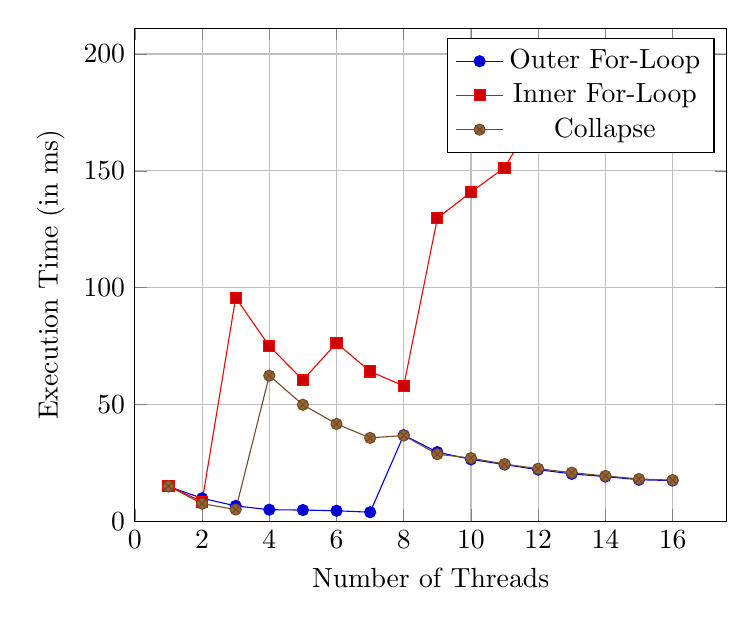
\begin{tikzpicture}
            \begin{axis}[
                title={},
                width=0.75\textwidth,
                xlabel={Number of Threads},
                ylabel={Execution Time (in ms)},
                xmin=0,
                ymin=0,
                grid=major
            ]
                \addplot coordinates {
                    (1,14.9234)(2,9.8524)(3,6.59485)(4,4.95885)(5,4.82065)(6,4.5133)(7,3.89165)(8,36.8866)(9,29.6062)(10,26.494)(11,24.2738)(12,22.0962)(13,20.3089)(14,19.1307)(15,17.7853)(16,17.4446)
                };
                \addlegendentry{Outer For-Loop}

                \addplot coordinates {
                    (1,15.243)(2,8.3793)(3,95.7094)(4,74.9772)(5,60.4569)(6,76.2988)(7,64.1251)(8,57.9691)(9,129.706)(10,140.856)(11,151.381)(12,175.358)(13,191.842)(14,171.761)(15,167.276)(16,189.499)
                };
                \addlegendentry{Inner For-Loop}       

                \addplot coordinates {
                    (1,15.0915)(2,7.557)(3,5.04065)(4,62.3426)(5,49.8704)(6,41.6652)(7,35.6859)(8,36.7201)(9,28.7093)(10,27.0565)(11,24.5003)(12,22.5038)(13,20.8165)(14,19.4369)(15,18.1129)(16,17.6074)
                };
                \addlegendentry{Collapse}
            \end{axis}
        \end{tikzpicture}
        \caption{Grayscale Performance Tests dice.png}
    \end{figure}
\end{center}

\end{frame}

\begin{frame}
    \frametitle{Grayscale - Ergebnisse 2}

    \begin{itemize}
        \item dice\_large.png
        \item 1754 x 1554
        \item 1.5 MB
    \end{itemize}

    \hfill
    \hrule
    \hfill

    \begin{figure}[H]
        \centering
    
        \includegraphics[width=0.30\textwidth]{images/dice_large.png}
        \includegraphics[width=0.30\textwidth]{images/results/grayscale-cv.dice_large.png}
        \includegraphics[width=0.30\textwidth]{images/results/grayscale-my.dice_large.png}

        
        \begin{center}
            \caption{Grayscale results of OpenCV (middle) and self-implemented  Algorithm (right)}            
        \end{center}

        \label{fig:grayscale2}
    \end{figure}
\end{frame}

\begin{frame}
    \frametitle{Grayscale - Performance 2}

    \begin{center}
    \begin{figure}[H]
        \centering

        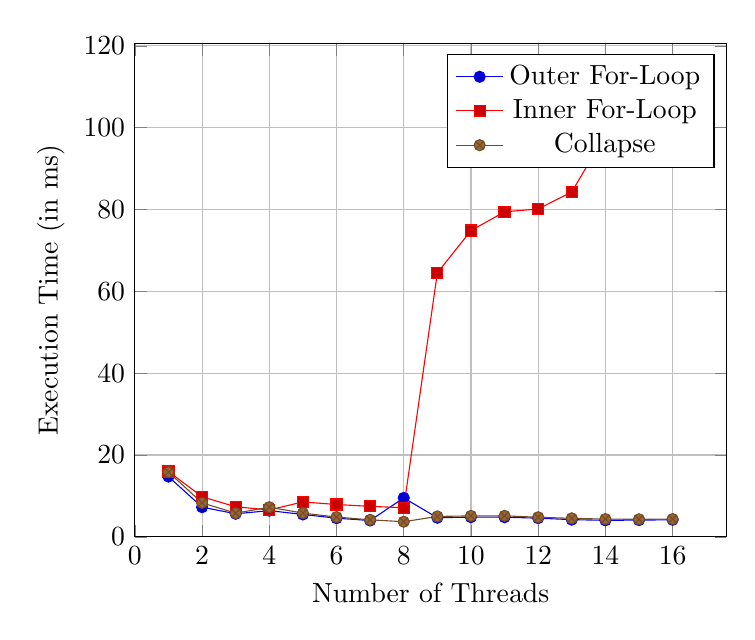
\begin{tikzpicture}
            \begin{axis}[
                title={},
                width=0.75\textwidth,
                xlabel={Number of Threads},
                ylabel={Execution Time (in ms)},
                xmin=0,
                ymin=0,
                grid=major
            ]
                \addplot coordinates {
                    (1,14.7211)(2,7.25495)(3,5.6363)(4,6.40325)(5,5.47325)(6,4.55525)(7,3.98965)(8,9.51975)(9,4.6724)(10,4.81735)(11,4.7994)(12,4.5654)(13,4.20095)(14,4.03585)(15,4.0938)(16,4.16465)
                };
                \addlegendentry{Outer For-Loop}

                \addplot coordinates {
                    (1,15.9672)(2,9.79695)(3,7.347)(4,6.57375)(5,8.53395)(6,7.9008)(7,7.455)(8,7.12075)(9,64.5109)(10,74.8451)(11,79.4215)(12,80.1279)(13,84.2831)(14,98.2654)(15,96.7823)(16,109.546)
                };
                \addlegendentry{Inner For-Loop}       

                \addplot coordinates {
                    (1,15.8111)(2,8.30245)(3,5.78465)(4,7.24315)(5,5.80145)(6,4.82905)(7,4.161)(8,3.69605)(9,4.9833)(10,5.11935)(11,5.1344)(12,4.7873)(13,4.5233)(14,4.33805)(15,4.2893)(16,4.3391)
                };
                \addlegendentry{Collapse}
            \end{axis}
        \end{tikzpicture}
        \caption{Grayscale Performance Tests dice\_large.png}
    \end{figure}
\end{center}

\end{frame}

\begin{frame}
    \frametitle{Grayscale - Ergebnisse 3}

    \begin{itemize}
        \item pnglogo-blk.png
        \item 1024 x 768
        \item 516 KB
    \end{itemize}

    \hfill
    \hrule
    \hfill

    \begin{figure}[H]
        \centering
    
        \includegraphics[width=0.30\textwidth]{images/pnglogo-blk.png}
        \includegraphics[width=0.30\textwidth]{images/results/grayscale-cv.pnglogo-blk.png}
        \includegraphics[width=0.30\textwidth]{images/results/grayscale-my.pnglogo-blk.png}

        
        \begin{center}
            \caption{Grayscale results of OpenCV (middle) and self-implemented  Algorithm (right)}            
        \end{center}

        \label{fig:grayscale3}
    \end{figure}
\end{frame}

\begin{frame}
    \frametitle{Grayscale - Performance 3}

    \begin{center}
    \begin{figure}[H]
        \centering

        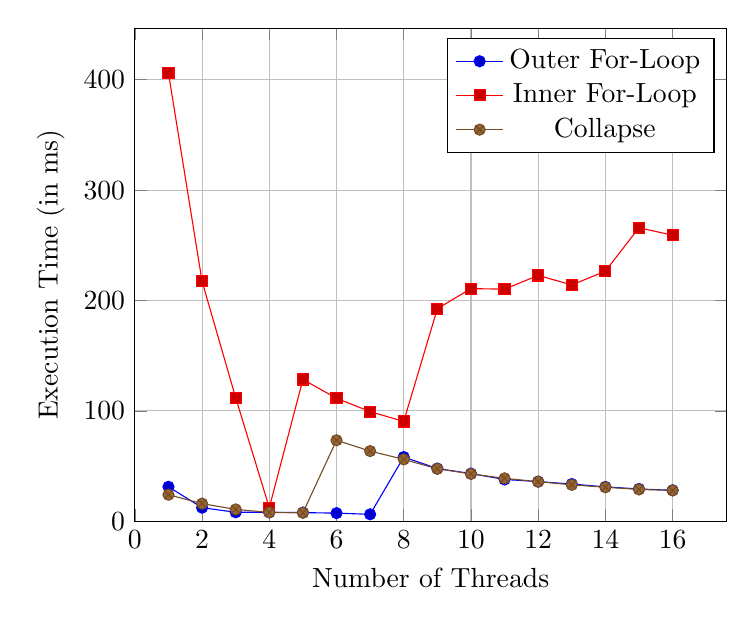
\begin{tikzpicture}
            \begin{axis}[
                title={},
                width=0.75\textwidth,
                xlabel={Number of Threads},
                ylabel={Execution Time (in ms)},
                xmin=0,
                ymin=0,
                grid=major
            ]
                \addplot coordinates {
                    (1,31.2605)(2,12.3476)(3,8.17925)(4,8.15845)(5,7.901)(6,7.3853)(7,6.33095)(8,58.2227)(9,47.7963)(10,43.2362)(11,37.9023)(12,35.9582)(13,33.7485)(14,31.185)(15,29.2952)(16,28.0915)
                };
                \addlegendentry{Outer For-Loop}

                \addplot coordinates {
                    (1,406.043)(2,217.313)(3,111.939)(4,12.3023)(5,128.511)(6,111.441)(7,99.3506)(8,90.4608)(9,192.601)(10,210.794)(11,210.268)(12,222.735)(13,214.113)(14,226.578)(15,265.97)(16,259.109)
                };
                \addlegendentry{Inner For-Loop}       

                \addplot coordinates {
                    (1,24.0952)(2,16.0462)(3,10.7771)(4,8.0282)(5,7.75735)(6,73.4093)(7,63.6226)(8,56.107)(9,47.5841)(10,42.9433)(11,38.9119)(12,35.9038)(13,33.0421)(14,30.8513)(15,28.8692)(16,27.9851)
                };
                \addlegendentry{Collapse}
            \end{axis}
        \end{tikzpicture}
        \caption{Grayscale Performance Tests pnglogo-blk.png}
    \end{figure}
\end{center}

\end{frame}